\begin{itemize}
        \item \begin{tt} db.media.find() \end{tt} \newline
        Cette requête trouve tous les éléments de la collection "media". Cette collection appartient à la base de donnée "library".

        \item \begin{tt} db.media.find(\{Artist:"Nirvana"\}) \end{tt} \newline
        Cette requête trouve tous les documents ayant pour valeur "Nirvana" associée à leur champ artiste.
        
        \item \begin{tt} db.media.find(\{Artist:"Nirvana"\},\{Title: 1\}) \end{tt} \newline
        Cette requête trouve tous les documents ayant pour valeur "Nirvana" dans leur champ artiste et n'affiche que le champ "Title" et "\_id" grâce à une projection\textsuperscript{1}.
        
        \item \begin{tt} db.media.find(\{Artist:"Nirvana"\},\{Title:0\}) \end{tt} \newline
        Cette requête trouve tous les documents ayant pour valeur "Nirvana" dans leur champ artiste sans afficher leur champ "title".
        
        \item \begin{tt} db.media.find(\{"Tracklist.Title":"In Bloom"\}) \end{tt} \newline
        Cette requête trouve tous les documents ayant un sous document de titre "in Bloom".

        \item \begin{tt} db.media.findOne() \end{tt} \newline
        findOne retourne le premier document respectant les conditions passées en paramètre (aucune conditions dans ce cas). Elle renvoie donc le premier document inséré dans la collection.

    \end{itemize}
    
    \begin{block}{Note}
         La projection\textsuperscript{1} est le deuxième argument optionel de la méthode .find() il est de forme "field": 1/0 et permet de spécifier les champs que l'on veut récupérer. Par défaut le champ \_id s'affiche si on ne préscise pas {"\_id": 0} 
    \end{block}

{\let\thefootnote\relax\footnotetext{\textsuperscript{1}\textit{Usages and examples of \href{http://docs.mongodb.org/manual/reference/operator/projection/positional/}{\$(projection)}}}}

    \begin{itemize}
        \item \begin{tt} db.media.find().sort(\{Title:1\}) \end{tt} \newline
        La méthode .find() retourne un objet de type "Object Cursor". En applicant la méthode sort on ordonne le résultat de la requête. Ici on affiche tous les documents de la collection media dans la base Library par ordre croissant. 
        \item \begin{tt} db.media.find().sort(\{Title:-1\}) \end{tt} \newline
        Ici on affiche tous les documents de la collection media dans la base Library par ordre décroissant.
        \item \begin{tt} db.media.find().limit(10) \end{tt} \newline
        Ici on affiche les 10 premiers documents de la collection.
        
        \item \begin{tt} db.media.find().pretty() \end{tt} \newline
        La commande .pretty() permet d'agencer le JSON qui résulte de la requête pour une meilleur comprehension du résultat.
    \end{itemize}
    
    \begin{figure}[h!]
    \centering
    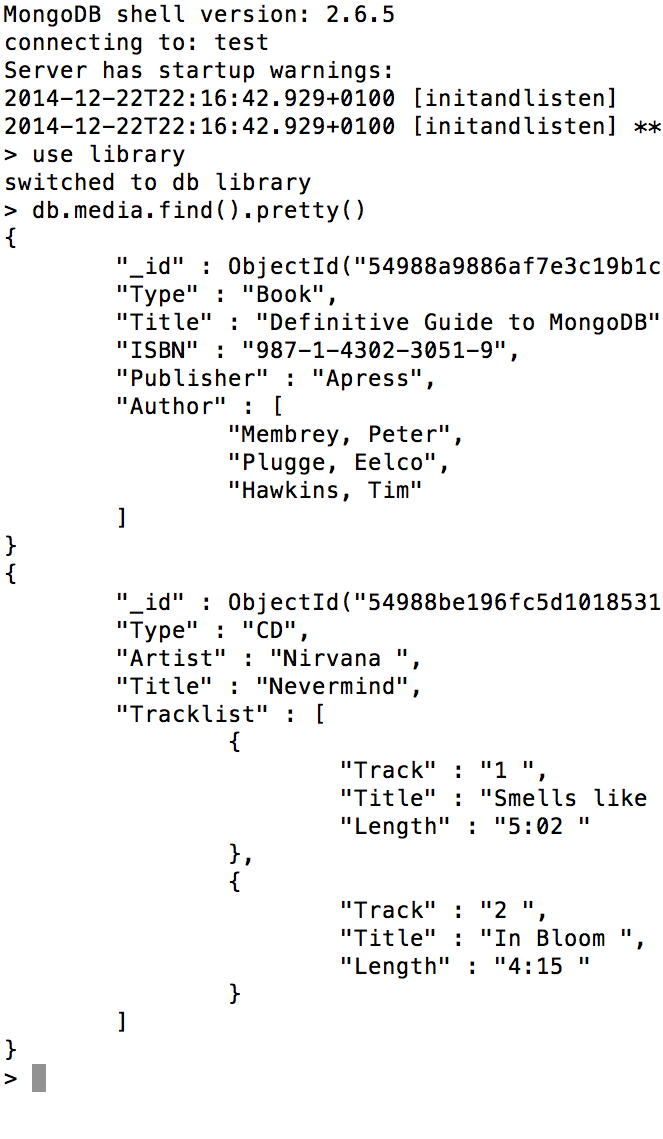
\includegraphics[scale=0.6]{img/pretty.png}
    \caption{Exemple d'utilisation de la méthode .pretty() en console}
    \end{figure}
    
    \par
        Ce comportement est automatiquement géré par l'interface RoboMongo\textsuperscript{2}. Après cette première partie sur les requêtes nous continurons le TP sur RoboMongo et laisseront tomber la consol.   

{\let\thefootnote\relax\footnotetext{\textsuperscript{2} \textit{RobotMongo, the MongoDB management tool. \href{http://robomongo.org}{http://robomongo.org}}}}
    \begin{itemize}
        \item \begin{tt} db.media.find().skip(20) \end{tt} \newline
        On recupère tous les documents à partir du 20 éléments du curseur renvoyé par .find(). La méthode .skip(n) permet de d'ignorer un certain nombre de résultats.
        \item \begin{tt} db.media.find().sort (\{Title:-1\}).limit(10).skip(20) \end{tt} \newline
        On obtient les 10 résultats à partir du 20ème sur la liste des documents par ordre décroissant des titres.
    \end{itemize}
    \begin{block}{Remarque}
        On peut trouver cette dernière requête particulièrement contre intuitive. on pourrait penser que db.media.find().sort(\{Title:-1\}).limit(m) renvoie une liste de m éléments et que l'on y applique .skip(n) pour passer les n premiers. Au lieu de celà on peut inverser les instructions .limite() et .skip(), on a le même résultat.
    \end{block}